\section{YARN-Modell}\label{sec:yarnModel}

\begin{figure}
	\centering
	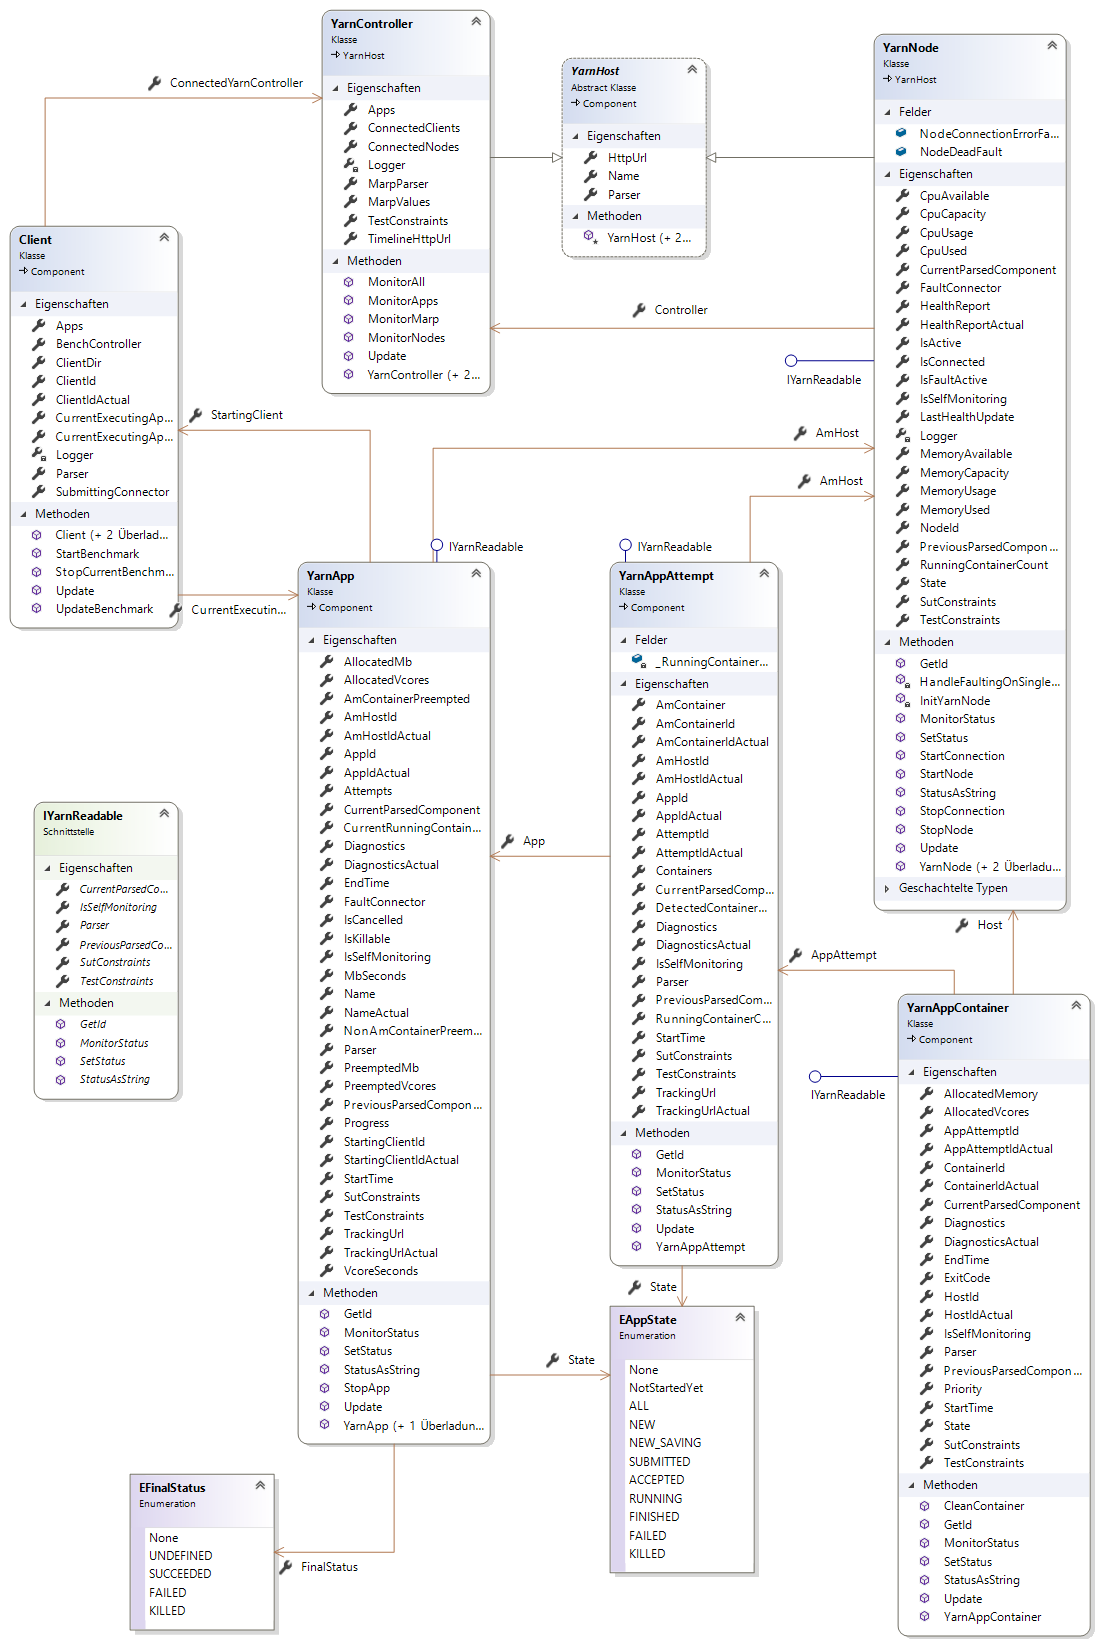
\includegraphics[width=\columnwidth]{./images/yarnModel.png}
	\caption[Aufbau des YARN-Modells]{Aufbau des YARN-Modells. Das Modell wurde mithilfe des Klassendiagramm-Designers in Visual Studio 2017 erstellt. Daher werden die aus Listen bestehenden Gegenassoziationen zu den Eigenschaften \texttt{YarnAppAttempt.App} (\texttt{YarnApp.Attempts}) und \texttt{YarnAppContainer.AppAttempt} (\texttt{YarnAppAttempt.Containers}) nicht im Diagramm angezeigt.}
	\label{fig:yarnModel}
\end{figure}

\autoref{fig:yarnModel} beschreibt im Grunde bereits das gesamte von \sS verwendete YARN-Modell. Enthalten sind alle hier relevanten Komponenten sowie deren Eigenschaften. Die abstrakte Basisklasse \texttt{YarnHost} stellt die Basis für alle Hosts des Clusters dar, also dem \texttt{YarnController} mit dem \ac{RM}, und dem \texttt{YarnNode}, was einen Node darstellt, auf dem die Anwendungen bzw. deren Container ausgeführt werden.